%---------------------导言区---------------------------%
\documentclass[12pt,a4paper,UTF8]{ctexart}
	%10pt：正文字体为12pt，缺省为10pt；各层级字体大小会根据正文字体自动调整
	%a4paper：纸张大小a4；
	%UTF8：中文要求
\usepackage{geometry}%用于设置上下左右页边距
	\geometry{left=2.5cm,right=2.5cm,top=3.2cm,bottom=2.8cm}
\usepackage{xeCJK}
\usepackage{amsmath}
\usepackage{paralist}
\usepackage{enumerate}
\usepackage{booktabs}
\usepackage{multirow}
\usepackage{graphicx}
\usepackage{subfig}
\usepackage{setspace}
\usepackage{listings}
\usepackage{lastpage}
\usepackage{hyperref}
\usepackage{pdfpages}

%xeCJK：中文字体（如楷体，作者和机构需要用到）的设置
	%amsmath：数学公式
	%paralist，enumerate：自定义项目符号
	%booktabs：三线图，论文常用的表格风格
	%multirow：复杂表格
	%graphicx，float: 插入图片
	%subfig：并排排版图片、竖向排版图片
	%setspace：设置行间距等功能
	\setlength{\parindent}{2em}%正文首行缩进两个汉字
	%listings:用于排版各种代码；比如matlab的代码
	\lstset{language=Matlab}%matlab代码
	%lastpage:获取总页数;
	%hyperref:超链接,和lastpage搭配.
\usepackage{fancyhdr}
	%fancyhdr：一个很强大的宏包，用于自定义设计页面风格并命名以供调用。
	\pagestyle{fancy}
	\rhead{微波电子自旋实验}
	\lhead{近代物理实验~~~实验报告}
	\cfoot{Page \thepage/\pageref{LastPage}}  %当前页\总页数
	\rfoot{\today}
		%分别是右页眉、左页眉、中页脚、右页脚
	\renewcommand{\headrulewidth}{0.4pt}
	\renewcommand{\theenumi}{(\arabic{enumi})}

%%%%%%%%%%%%%%%%%%%%%%%%%%%%%%%%%%%%%%%%%%%%%%%%%%%%%%%%%%
%%%%%%%%%%%%%%%%%%%%%%%%%正文开始%%%%%%%%%%%%%%%%%%%%%%%%%%
%%%%%%%%%%%%%%%%%%%%%%%%%%%%%%%%%%%%%%%%%%%%%%%%%%%%%%%%%%

\begin{document}

%%begin-------------------标题与信息-----------------------%%

%%标题
\begin{center}
\LARGE\textbf{微波电子自旋实验}
\end{center}

%%信息
\begin{doublespacing}
	%doublespacing：手动两倍行距
	\begin{tabular}{lr}
	 & \\
	 {实验人姓名：徐殊行~23343071} & {合作者姓名：王志超~23343062}\\
	 {实验时间：2025年5月16日/23日} & {室温：24$^{\circ}$C~相对湿度：69\%}
	
	\end{tabular}
\end{doublespacing}

%%-------------------中英文摘要-----------------------%%
\begin{abstract}
    本实验通过微波电子自旋共振实验仪测量DPPH中电子的朗德因子g和共振线宽，并计算得到弛豫时间。
    本实验利用FD-ESR-C型微波电子自旋共振实验仪，以有机自由基DPPH（二苯基-苦基肼基）为研究样品，观测并分析其电子自旋共振（ESR）现象。
    通过调节恒定磁场与微波频率，记录样品在共振条件下的吸收信号，从而测定其朗德因子 \(g\) 及共振线宽。
    实验过程中探讨了磁场均匀性、扭波导作用以及不同共振线型的物理意义，并结合理论公式 \(h\nu = g\mu_B B_0\) 进行了数据计算与分析。
    实验结果验证了电子具有自旋磁矩这一量子特性，进一步加深了对量子磁共振机制的理解。

	\noindent \textbf{关键词：} 微波电子自旋共振；DPPH；朗德因子；塞曼分裂；共振线型
		
\end{abstract}
	
\renewcommand{\abstractname}{Abstract}

\begin{abstract}
    In this experiment, we employed the FD-ESR-C type microwave electron spin resonance (ESR) spectrometer to investigate the ESR phenomenon of the organic free radical DPPH (diphenylpicrylhydrazyl).
    By adjusting the static magnetic field and microwave frequency, we observed the resonance absorption signal and measured the sample's Landé \(g\)-factor and resonance linewidth.
    The effects of magnetic field uniformity, the function of the twist waveguide, and the physical significance of different resonance line shapes were also discussed.
    Based on the resonance condition \(h\nu = g\mu_B B_0\), we performed data analysis and theoretical calculations.
    The experimental results confirm the intrinsic magnetic moment associated with electron spin and deepen our understanding of quantum magnetic resonance mechanisms.

	\noindent \textbf{Keywords: }Microwave electron spin resonance; DPPH; Landé factor; Zeeman splitting; Resonance line shape
\end{abstract}

%%-------------------正文部分-----------------------%%

\subsection*{【实验目的】}
\begin{enumerate}[(1)]
    \item 了解电子自旋共振现象及物理原理；
    \item 学习用微波频段检测电子自旋共振的技术方法；
    \item 测量DPPH中电子的朗德因子g和共振线宽。
\end{enumerate}

\subsection*{【实验原理】}

\subsubsection*{原子核结构}
原子由质量主要集中在原子核（由质子和中子构成）和环绕其周围的电子组成。
典型原子半径约为 \(10^{-10}\)\,m，而原子核尺寸仅在 \(10^{-15}\!-\!10^{-14}\)\,m 量级，因此原子质量几乎全部由核子承担。
电子质量 \(m_e = 9.1094\times10^{-31}\,\mathrm{kg}\)，电荷量 \(\lvert e\rvert = 1.6022\times10^{-19}\,\mathrm{C}\)；
质子质量约为电子的 1836 倍。电子在原子中既有轨道运动（产生轨道角动量和轨道磁矩），又具有内秉的自旋角动量和自旋磁矩，是本实验研究的核心对象。

\subsubsection*{电子自旋磁矩和跃迁能量关系}
电子自旋量子数 \(s=\tfrac12\)，其角动量大小
\[
|\boldsymbol{S}| = \sqrt{s(s+1)}\,\hbar = \tfrac{\sqrt3}{2}\,\hbar,
\]

在外加磁场 \(\boldsymbol{B}_0\)（取 \(z\) 方向）作用下，自旋分量量子化为
\[
S_z = m_s\hbar,\quad m_s = \pm\tfrac12.
\]

电子自旋磁矩 \(\boldsymbol{\mu}_s\) 与角动量 \(\boldsymbol{S}\) 的关系为
\[
\boldsymbol{\mu}_s = \gamma_s\,\boldsymbol{S}
\quad\text{或}\quad
\mu_{s z} = \gamma_s\,m_s\hbar,
\]

其中旋磁比 \(\displaystyle \gamma_s = \frac{g_s e}{2m_e}\)，自旋朗德因子 \(g_s\approx2\)。以玻尔磁子 \(\mu_B = \frac{e\hbar}{2m_e}\) 为单位，则
\[
\mu_{sz} = g_s\,m_s\,\mu_B.
\]

在磁场中，电子两自旋态能级差（塞曼分裂）为
\[
\Delta E = g_s\,\mu_B\,B_0.
\]

当施加频率 \(\nu\) 的交变场满足共振条件
\[
h\nu = \Delta E = g_s\,\mu_B\,B_0,
\]

电子可发生自旋跃迁并吸收能量，从而在示波器上观测到共振吸收信号。

\subsubsection*{实验 DPPH 样品介绍}
本实验选用有机自由基二苯基-苦基肼基（DPPH）作为顺磁样品：DPPH 分子中仅第二个氮原子存在一个未成对电子，该电子无轨道角动量（\(l=0\)），仅有自旋角动量 \(s=\tfrac12\)，故其总朗德因子
\[
g \approx 2.0036.
\]
将样品置于约 \(0.3\)\,T 的恒磁场中，代入
\[
\nu = \frac{g\,\mu_B}{h}\,B_0
\approx 2.0036\cdot\frac{0.9274\times10^{-23}}{6.626\times10^{-34}}\times0.3
\approx 8.4\times10^9\,\mathrm{Hz},
\]
可知共振频率在 \(10^4\)\,MHz 级别，属于微波波段。通过测量共振频率与共振场强，可反算样品 \(g\) 因子；谱线宽度又可反映样品的自旋–晶格和自旋–自旋弛豫过程。

\subsection*{【实验仪器】}
\begin{table}[h!]
	\centering
	\begin{tabular}{|p{5cm} p{4cm} p{5cm}|}
		\hline
		仪器名称 & 型号 & 参数 \\
		\hline\hline
		微波电子自旋共振实验仪 & FD-ESR-C & - \\
		示波器 & MDO4034C &  350 MHz \\
		\hline		
	\end{tabular}
	\caption{实验仪器及参数}
	\label{tab:instruments}
\end{table}

\subsection*{【实验内容】}
\begin{enumerate}
    \item 理解实验物理原理和实验技术原理；认真阅读《微波段电子自旋共振实验仪》使用说明书；确认实验系统各仪器（设备）之间连接无误。
    \item 使用示波器观察信号变化进行实验系统调节：
    \begin{itemize}
            \item 检波二极管输出 $\leftrightarrow$ 示波器"CH2"
            \item "相位调节"输出 $\leftrightarrow$ 示波器"CH1"
    \end{itemize}
    \item 示波器CH2为DC（直接耦合）输入，CH1为AC（交流耦合）输入且为同步触发信号。选择适当量程，并记录CH2接地时信号线在显示屏位置，即"零线"。
    \item 反复调节终端负载和双T调配器的短路活塞（达到输出匹配），使检波器输出信号尽可能远离"零线"（信号幅值最大），即波导管内形成微波驻波。
    \item 测量微波频率。本实验使用"吸收式"频率计测量波导管中微波频率。调节频率计的调谐机构至产生谐振，对应于检波器输出最小时谐振机构读数即为微波频率。
    \item 测量波导波长。将终端负载短路活塞调至最远离起点第一次最大输出信号处，记录短路面位置读数；移动短路活塞，每出现最大输出信号均记录短路面位置读数。
    \item 示波器CH2改为AC（交流耦合）输入模式，且选择适当量程。终端负载短路活塞置于最靠近起点的最大检波信号处。插入样品，使"扫场电源"输出最大，缓慢调节"电磁铁励磁电源"电位器改变励磁电流，观察检波器输出信号变化直至出现磁共振吸收信号。细调短路活塞使共振吸收信号尽可能对称。
    \item 改变 ESR 实验仪的"移相器"相位和"扫场电源"输出，观测分析磁共振吸收信号变化，从而确定系统最佳实验条件。
    \item 取出样品，用高斯计测量样品所在处的磁场强度。
    \item 再次插入样品，微调ESR实验仪励磁电路和终端负载短路活塞使再次获得尽可能对称信号。重复步骤（9）。
    \item 重复步骤（10），分析朗德因子。注意正确运用实验误差分析方法。
    \item 拟定观测电子自旋共振吸收峰半高宽方法，实验记录并分析之。
    \item （可选内容）逐点记录分析电子自旋共振吸收线形。将检波器输出接电流表，由小至大逐渐改变励磁电流强度，观察记录两者读数。如何正确分析实验结果？
    \item 实验完毕，
    \begin{enumerate}[(1)]
        \item 将仪器各旋扭复位并切断电源；
        \item 将仪器和实验资料摆放整齐；
        \item 清洁桌面，不要遗留个人用品。经任课老师确认并在《近代物理实验室仪器设备登记表》上签字方可离开实验室。
    \end{enumerate}
\end{enumerate}

\subsection*{【实验过程和数据处分析处理】}
仔细阅读上述实验过程，并检查实验仪器完整可用之后我们开始实验。

\subsubsection*{标定电流和磁场关系}
首先在示波器上确认扫场波形如图\ref{fig:sweep_field}所示。

\begin{figure}[h!]
    \centering
    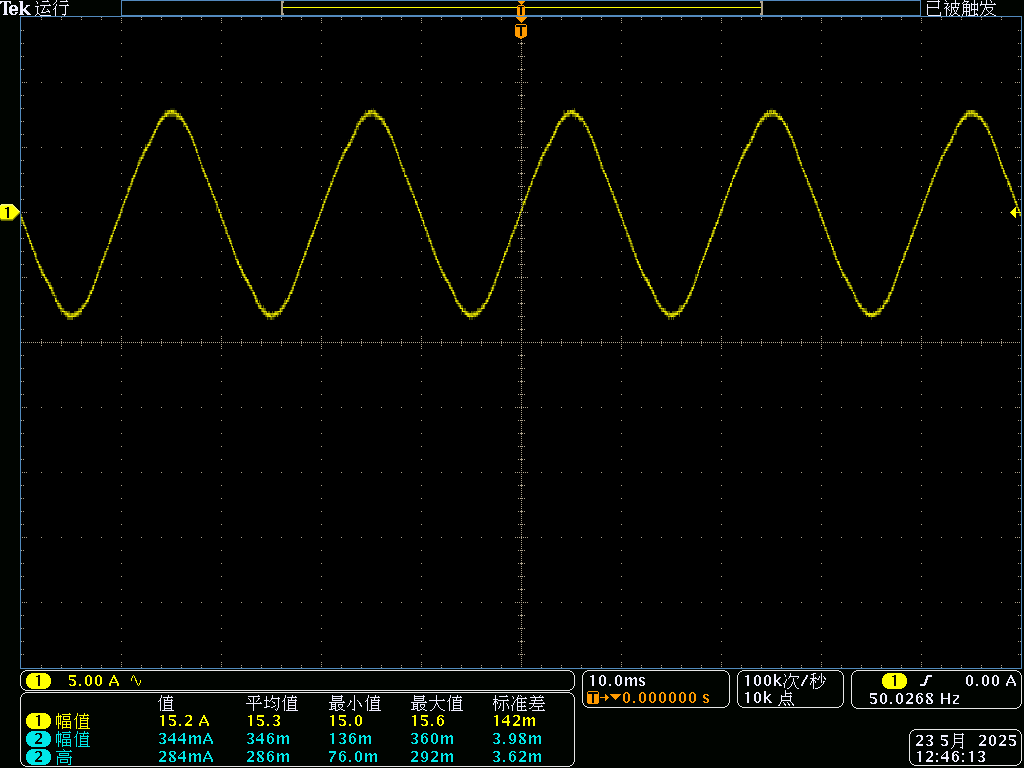
\includegraphics[width=0.5\textwidth]{扫场波形.png}
    \caption{扫场波形}
    \label{fig:sweep_field}
\end{figure}

我们为了方便后续处理，并计算g因子，我们首先标定电压和磁场的关系。

\begin{table}[h!]
    \centering
    \begin{tabular}{|c|c||c|c|}
        \hline
        励磁电压 $V$ & 磁场强度 $Gs$ & 励磁电流$V$ & 磁场强度 $Gs$ \\
        \hline\hline
        0.4 & 3174 & 2.8 & 3238 \\
        0.6 & 3180 & 3.0 & 3243 \\
        0.8 & 3185 & 3.2 & 3248 \\
        1.0 & 3190 & 3.4 & 3253 \\
        1.2 & 3196 & 3.6 & 3258 \\
        1.4 & 3201 & 3.8 & 3204 \\
        1.6 & 3206 & 4.0 & 3269 \\
        1.8 & 3211 & 4.2 & 3275 \\
        2.0 & 3216 & 4.4 & 3279 \\
        2.2 & 3221 & 4.6 & 3285 \\
        2.4 & 3227 & 4.8 & 3290 \\
        2.6 & 3232 & 5.0 & 3295 \\
        \hline
    \end{tabular}
    \caption{励磁电流与磁场强度对应关系}
    \label{tab:current_magnetic}
\end{table}

最后我们得到了拟合的结果，如图\ref{fig:current_magnetic}所示。

\begin{figure}[h!]
    \centering
    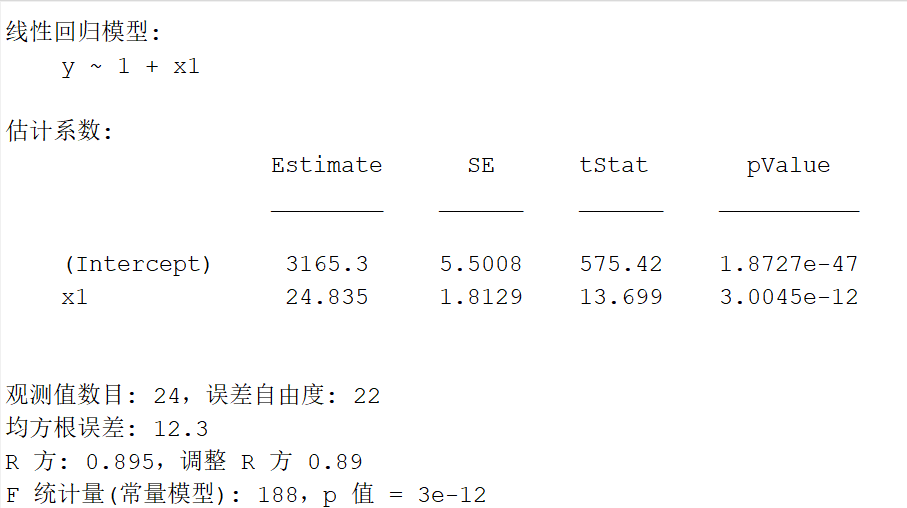
\includegraphics[width=0.5\textwidth]{拟合.png}
    \caption{励磁电流与磁场强度对应关系}
    \label{fig:current_magnetic}
\end{figure}

\subsubsection*{测量微波频率}
我们首先调节出共振信号如图\ref{fig:resonance_signal}所示。

\begin{figure}[h!]
    \centering
    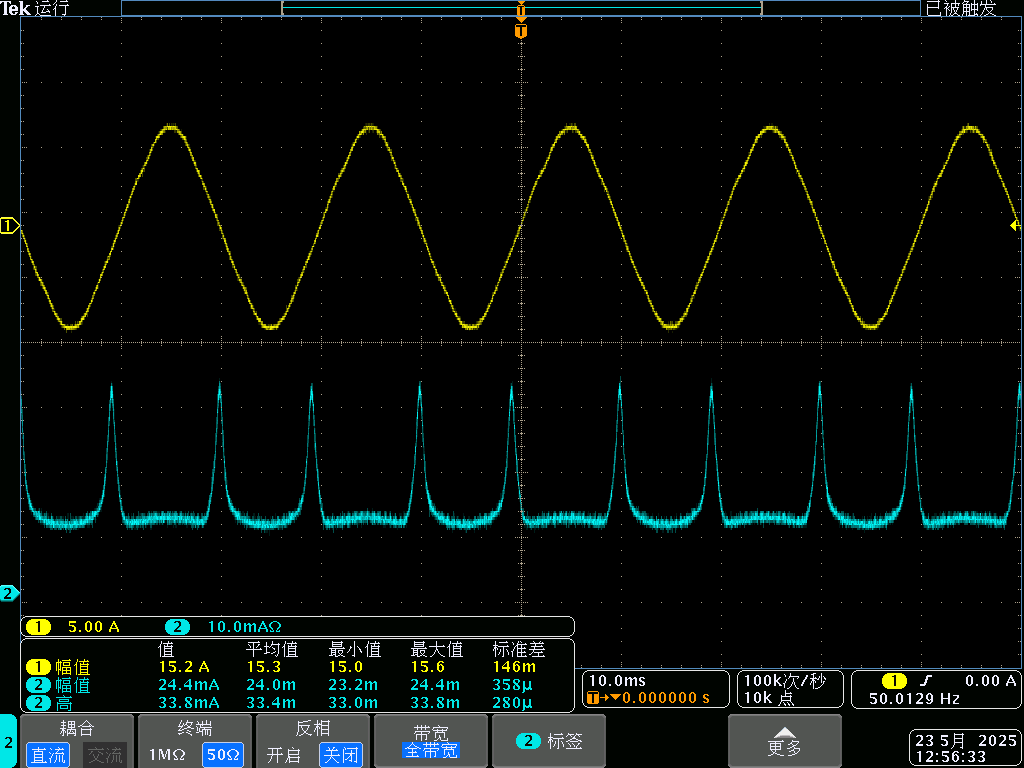
\includegraphics[width=0.5\textwidth]{共振信号2.png}
    \caption{共振信号}
    \label{fig:resonance_signal}
\end{figure}

随后使用"吸收式"频率计测量波导管中微波频率。
调节频率计的调谐机构至产生谐振，对应于检波器输出最小时谐振机构读数即为微波频率。

为了减小测量误差，我们在调节出谐振后，多次调节频率计的调谐机构，并记录每次谐振机构读数，最后取平均值作为微波频率。

\begin{table}[h!]
    \centering
    \begin{tabular}{|c|c|c|c|c|c|c|}
        \hline
        测量次数 & 1 & 2 & 3 & 4 & 5 & 6  \\
        \hline
        频率/GHz & 9.370 & 9.368 & 9.350 & 9.342 & 9.370 & 9.368 \\
        \hline
    \end{tabular}
    \caption{微波频率测量结果}
    \label{tab:frequency_measurement}
\end{table}

根据测量结果，我们计算得到微波频率的平均值为：
\begin{equation}
    f = \frac{9.370 + 9.368 + 9.350 + 9.342 + 9.370 + 9.368}{6} = 9.361 \text{ GHz}
\end{equation}

这个数值和讲义中给出的参考数值$9.36Ghz$相差不大，因此我们认为测量结果是较为准确的。

\subsubsection*{测量波导波长}
我们使用波导管中形成驻波的原理来测量波导波长。同样在调节出共振信号之后，我们多次调节短路活塞，并记录每次出现共振时短路活塞的位置，最后计算波导波长。
此时的励磁电压是$4.41V$，对应的磁场强度是$3275Gs$。

\begin{table}[h!]
    \centering
    \begin{tabular}{|c|c|c|}
        \hline
        测量次数 & $L_1/mm$ & $L_2/mm$ \\
        \hline\hline
        1 & 7.895 & 29.280 \\
        2 & 7.968 & 29.176 \\
        3 & 7.950 & 29.280 \\
        4 & 7.935 & 29.270 \\
        5 & 7.945 & 29.270 \\
        \hline
    \end{tabular}
    \caption{波导波长测量数据}
    \label{tab:waveguide_measurement}
\end{table}

随后我们根据公式
\begin{equation}
    \lambda = 2(L_2 - L_1)
\end{equation}
计算得到波导波长为$42.635mm$。

\subsubsection*{观察共振吸收信号}
按照实验步骤调节，我们得到的共振信号如图\ref{fig:resonance_signal}所示。

\begin{figure}[h!]
    \centering
    \subfloat[共振信号1]{
        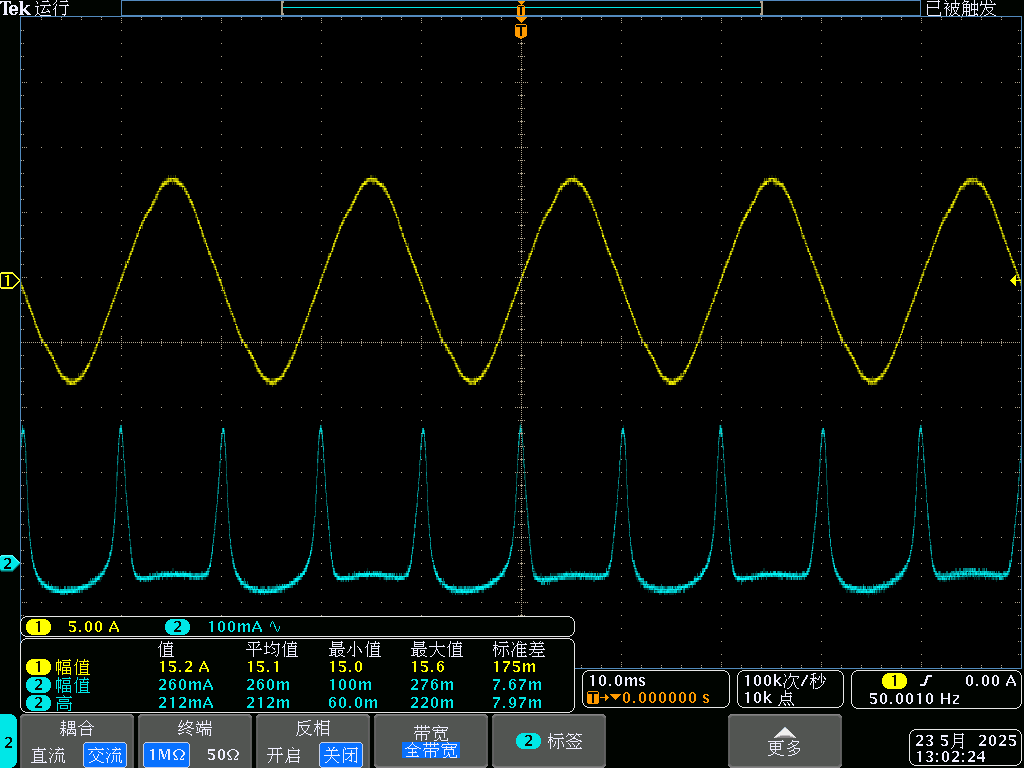
\includegraphics[width=0.45\textwidth]{共振信号3.png}
        \label{fig:resonance_signal1}
    }
    \hfill
    \subfloat[共振信号2]{
        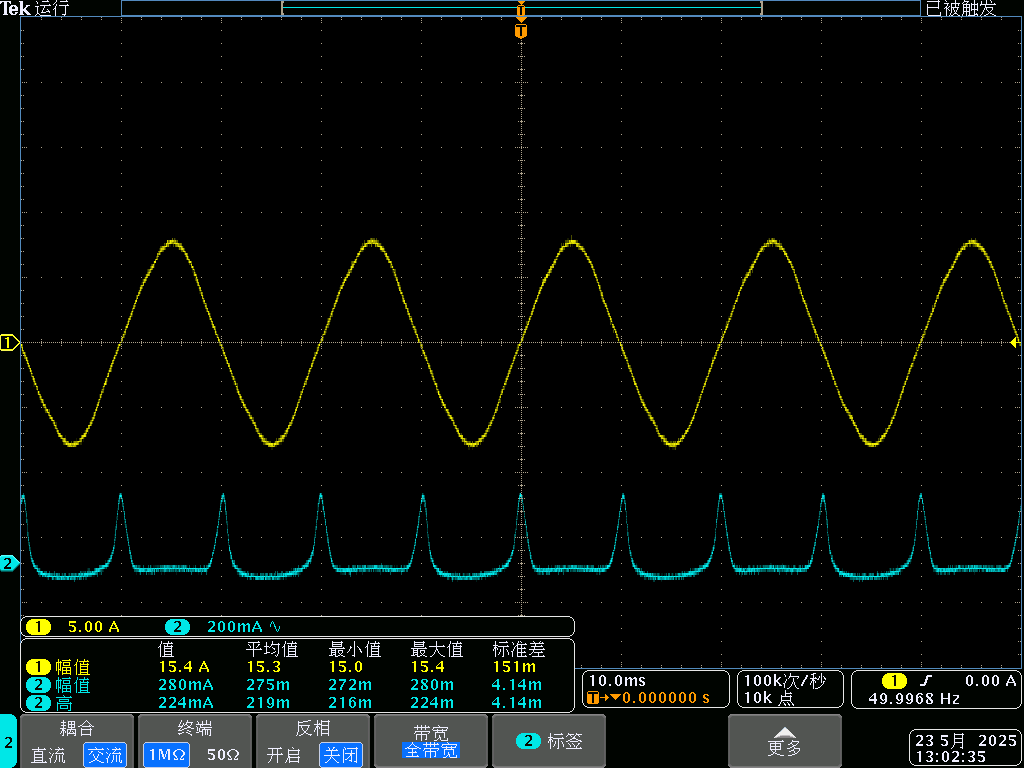
\includegraphics[width=0.45\textwidth]{共振信号4.png}
        \label{fig:resonance_signal2}
    }
    \caption{示波器共振信号}
    \label{fig:resonance_signal}
\end{figure}

之后我们将示波器调节到XY模式观察共振信号的李萨如图形，如图\ref{fig:lissajous_signal}所示。
\begin{figure}[h!]
    \centering
    \subfloat[示波器图像1]{
        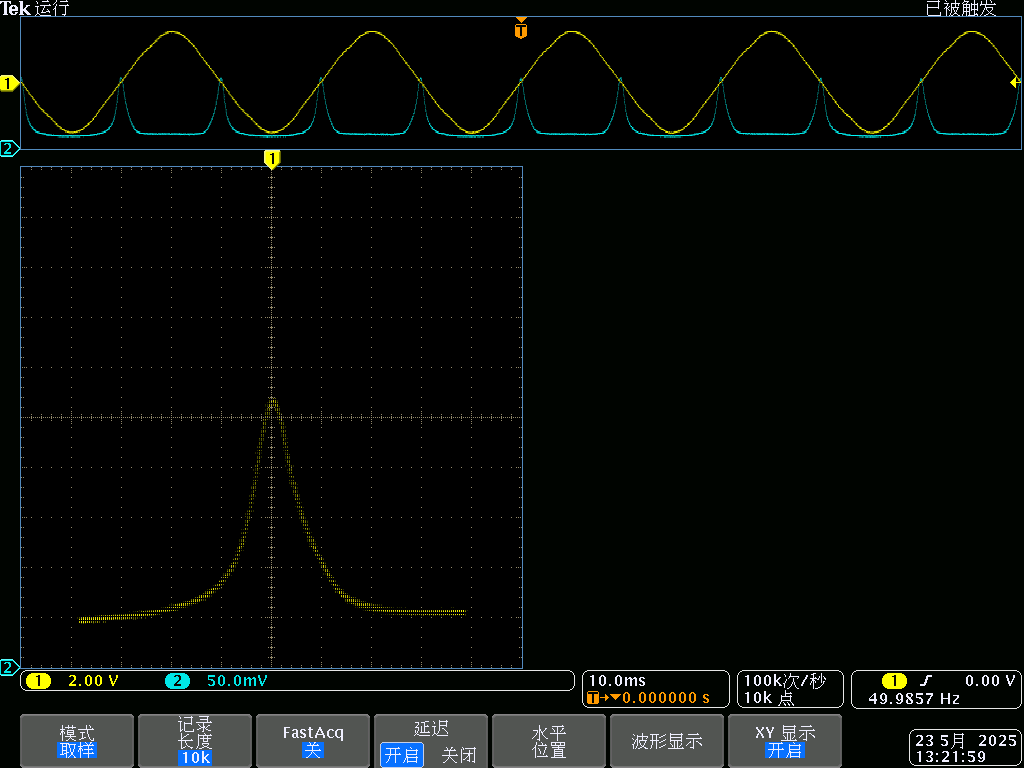
\includegraphics[width=0.45\textwidth]{李萨如图形.png}
        \label{fig:lissajous_signal1}
    }
    \hfill
    \subfloat[示波器图像2]{
        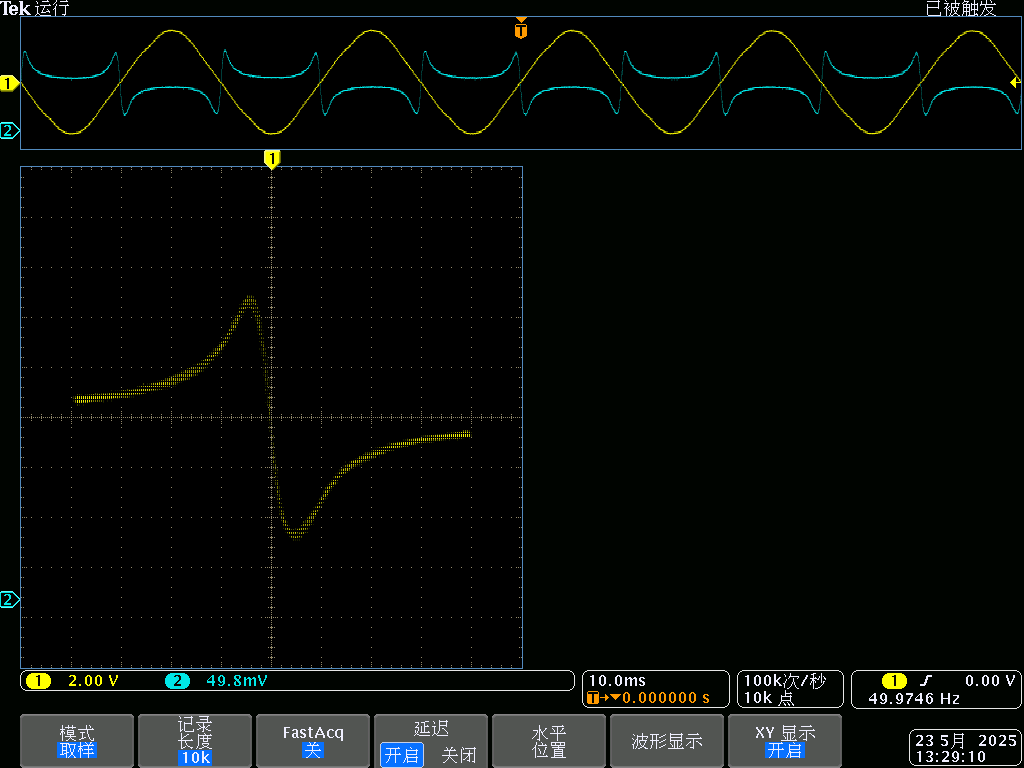
\includegraphics[width=0.45\textwidth]{洛伦兹峰.png}
        \label{fig:lissajous_signal2}
    }
    \caption{李萨如图形}
    \label{fig:lissajous_signal}
\end{figure}

\subsubsection*{计算朗德因子}
我们根据公式
\begin{equation}
    f = g \frac{\mu_{B}}{h}\,B_0
\end{equation}

代入我们计算得到的微波频率$9.361GHz$和励磁电压$5.40V$，对应磁场为$3299Gs$，计算得到朗德因子为$2.018$。

\paragraph{朗德因子误差分析}
在测量朗德因子的过程中，存在以下几个主要误差来源：

\begin{enumerate}[(1)]
    \item 样品位置误差：由于DPPH样品需要放置在磁场最均匀处才能获得最佳的共振信号，但实际操作中很难精确确定磁场最均匀的位置，这会导致测量到的磁场值与实际值存在偏差。
    
    \item 磁场测量误差：我们通过励磁电压与磁场的线性关系来间接测量磁场，但线性拟合本身存在一定的误差。特别是在拟合过程中，如果数据点分布不够均匀或存在异常点，都会影响拟合的准确性。
    
    \item 频率测量误差：使用频率计测量微波频率时，由于仪器本身的精度限制以及环境因素的干扰，测量结果可能存在一定的不确定性。特别是在高频段测量时，这种误差会更加明显。
\end{enumerate}

考虑到以上误差来源，我们计算得到的朗德因子$g=2.018$与理论值$g=2.0036$存在一定偏差。
这个偏差主要是由磁场测量和频率测量的误差共同导致的。为了减小误差，可以在实验过程中更加注意样品的放置位置，并多次测量取平均值来提高测量精度。

\subsubsection*{计算弛豫时间}
我们根据公式
\begin{equation}
    T_{2}=\frac{2}{\gamma\,\Delta B}
\end{equation}

其中$\gamma$是旋磁比，$\Delta B$是共振线宽。

通过处理示波器上读出的数据图\ref{fig:resonance_signal_matlab}所示并加以处理，我们可以得到共振线宽为$47.68Gs$。
并计算得到弛豫时间$T_2=1.18\times10^{-9}s$。

\begin{figure}[h!]
    \centering
    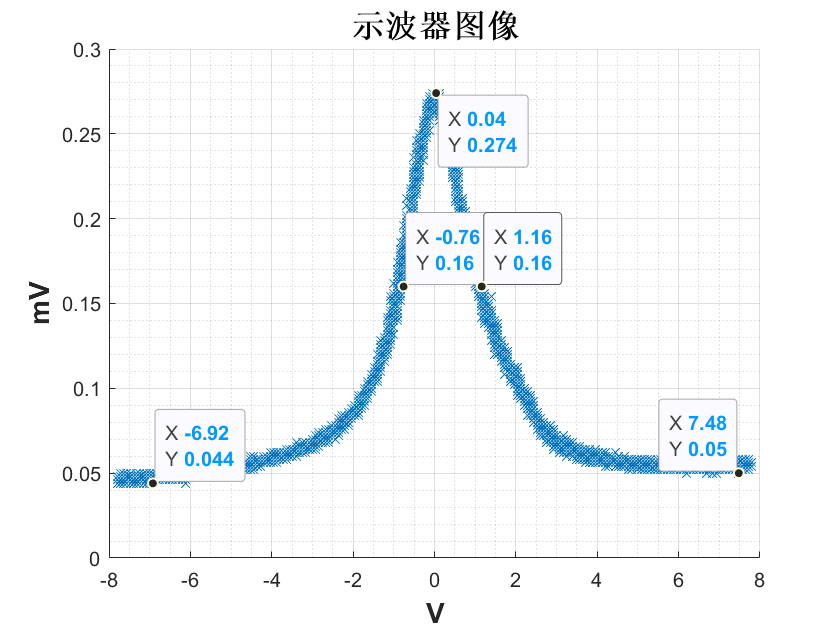
\includegraphics[width=0.65\textwidth]{示波器_matlab.png}
    \caption{示波器读数处理}
    \label{fig:resonance_signal_matlab}
\end{figure}

\paragraph{结果合理性分析}
我们得到的弛豫时间$T_2=1.18\times10^{-9}s$与理论预期值在数量级上是相符的。具体分析如下：

\begin{enumerate}[(1)]
    \item \textbf{数量级合理性}：电子自旋共振中的横向弛豫时间通常在纳秒量级，我们得到的结果$1.18\times10^{-9}s$正好处于这个范围内，说明测量结果是合理的。
    
    \item \textbf{与朗德因子的关系}：我们之前测量得到的朗德因子$g=2.018$与理论值$g=2.0036$的偏差在可接受范围内，这也间接支持了弛豫时间测量的可靠性。
    
    \item \textbf{误差来源分析}：
    \begin{itemize}
        \item 共振线宽的测量误差：示波器读数可能存在一定误差，特别是在确定半高宽时；
        \item 磁场均匀性影响：磁场不均匀会导致线宽测量值偏大，从而使计算得到的弛豫时间偏小；
        \item 样品纯度影响：DPPH样品的纯度会影响其弛豫特性。
    \end{itemize}
\end{enumerate}

总体而言，我们的测量结果在物理上是合理的，与理论预期相符。虽然存在一定误差，但考虑到实验条件和测量方法的限制，这个结果是可接受的。

\subsection*{【思考题】}

\subsubsection*{1. 磁场的均匀性对测量电子顺磁共振的驰豫有什么影响？}

磁场的均匀性直接影响共振信号的线型与宽度，进而影响对电子自旋弛豫过程的测量与分析。电子顺磁共振中的线宽主要受到两个方面的影响：

\begin{itemize}
  \item 一是电子系统自身的横向驰豫时间 \(T_2\)，它决定了理想情况下的自然线宽；
  \item 二是外部磁场的不均匀性会造成样品中不同区域的电子所感受到的共振场强 \(B_0\) 不同，导致共振频率在空间上出现分布，从而使得共振线被人为加宽（称为“非均匀展宽”）。
\end{itemize}

若磁场分布不均，会导致多个子区域的电子分别在略微不同的磁场处发生共振，测得的信号就是这些子信号的叠加结果，因而无法准确提取与 \(T_2\) 直接相关的谱线宽度，进而导致驰豫时间的估算误差增大。

因此，实验中需要保持磁场的高均匀性，以确保共振吸收峰集中，避免混入由外部不均匀性导致的伪展宽，提高对 \(T_2\) 的测量精度。

\subsubsection*{2. 实验中采用扭波导的意义是什么？}

本实验中采用扭波导的主要目的是\textbf{调整微波电磁场的偏振方向}，以便满足共振腔中磁场方向与微波场方向的正交要求。

根据实验装置的空间结构安排：
\begin{itemize}
  \item 外加静磁场（来自电磁铁）通常沿水平方向设置；
  \item 微波系统输出的电磁波其电场方向也位于水平方向；
  \item 然而激发电子自旋共振要求交变磁场与静磁场正交。
\end{itemize}

通过在波导中加入扭波导，可以实现波导结构的扭转，使输出端微波的磁场分量方向与恒稳磁场方向正交，从而保证共振条件满足。此外，扭波导无功耗、无能量衰减，是一种可靠且简便的方向调整装置。

\subsubsection*{3. 本实验中，波形有两种：对称与反对称线型。通过查询文献，了解出现这两种线型的原因及其物理意义。}

在电子自旋共振实验中，所观察到的共振信号可呈\textbf{对称线型}或\textbf{反对称线型}，两者对应不同的调制与检测方式：

\begin{itemize}
  \item \textbf{对称线型（Lorentzian 型）}：代表理想的共振吸收曲线，常见于直接探测微波功率的吸收强度。其中心对应共振条件被满足的位置，线宽反映横向驰豫时间 \(T_2\)。
  
  \item \textbf{反对称线型（导数型）}：实验中更常观测到的线型，是由于使用了磁场调制和锁相放大检波技术，输出的是吸收功率相对于磁场的导数信号，即 \(\frac{dP}{dB}\)。该方法有助于抑制噪声、增强信号清晰度。
\end{itemize}

此外，系统中存在的反射波或调配器调整不当也可能导致线型混合或偏离理想模型。

\textbf{物理意义上}：
\begin{itemize}
  \item 对称线型反映吸收功率本身；
  \item 反对称线型便于精确确定共振磁场位置、计算 \(g\) 因子和谱线宽。
\end{itemize}

\bibliography{ref.bib} %biblatex -> 'xelatex->pdfletax->xelatex'
\bibliographystyle{ieeetr}

\subsection*{【原始数据的记录】}
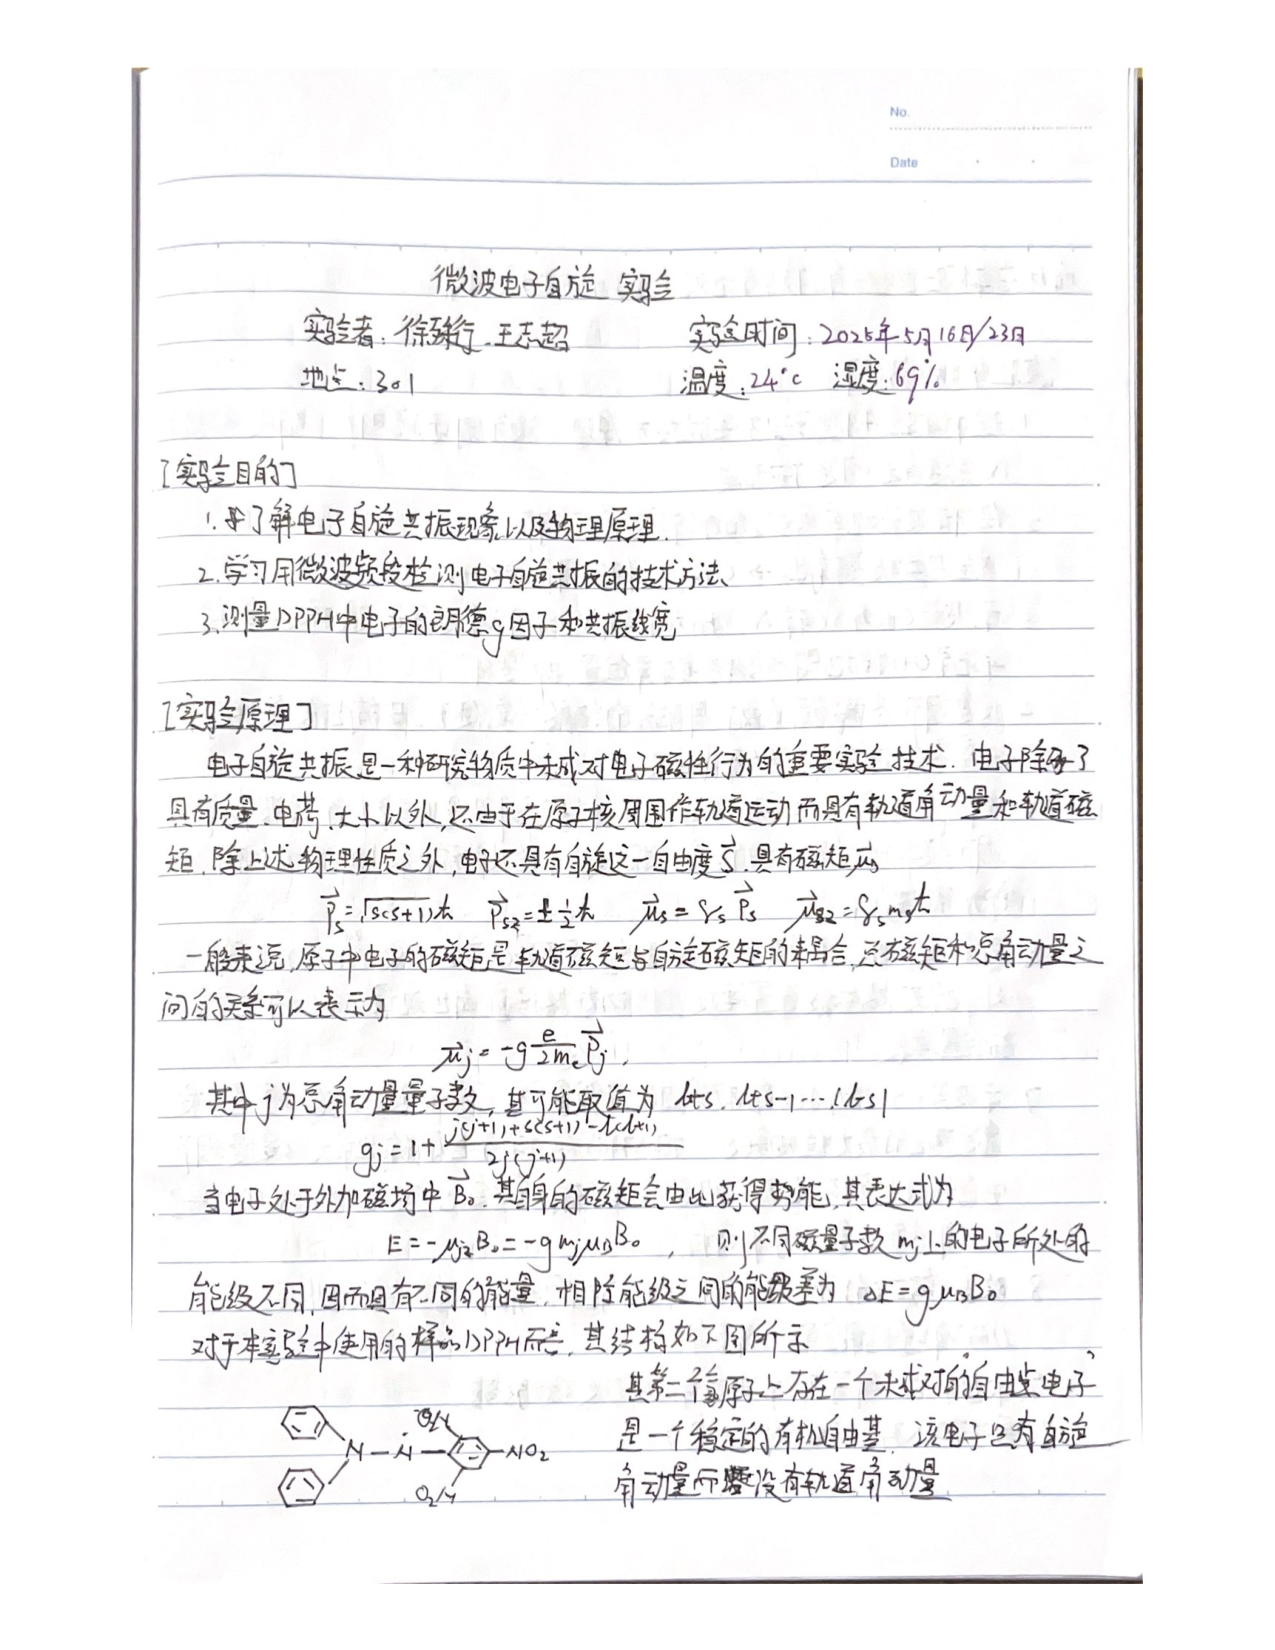
\includepdf[pages=-]{电子自旋scan.pdf}

\end{document}

